\section{Wellen}
\begin{itemize}
    \setlength\itemsep{1pt}
    \item Ausbreitungsphänomen von E und H
    \item Ausbreitungsgeschw. kleiner $c_0$
    \item raumzeitlicher Vorgang $cos(\omega t- \beta z)$
    \item Energie- ohne Materietransport
    \item Poyntingvektor $\vec{S}=\vec{E}\times\vec{H}$ Einheit[S]$= \dfrac{W}{m^2}$\\
          {\footnotesize Falls $\vec{E}\perp\vec{H}$ und $\vec{S}\perp\vec{E}$ und $\vec{S}\perp\vec{H}$}
\end{itemize}

\subsubsection*{Wellengleichung}
\makebox[0pt][l]{
    \begin{minipage}{\columnwidth}
        \centering
        \[
            \boxed{\vec{E} = \underbrace{E_0}_{\mathclap{\text{Amplitude}}}
            \cdot \overbrace{e^{-\alpha z}}^{\mathclap{\text{Dämpfung}}}
            \cdot \underbrace{cos(\omega t \overbrace{-}^{\mathclap{\text{positive z-Richtung}}} \beta z)}_\text{Zeit- und Raumabhängigkeit}}
        \]
        {\footnotesize Analog für H-Feld}
    \end{minipage}
}

\subsubsection*{Fortpflanzungskonstante $\gamma$}
\[\boxed{\underline{\gamma}=\alpha+j\beta}\]

$\alpha$ : Dämpfungskonstante [Np/m]

$\beta$ : Phasenkonstante [rad/m]

$v$ : Phasengeschwindigkeit [m/s]

$\lambda$ : Wellen [m]

\subsection{Ausbreitung}
\subsubsection{Allgemein}
\begin{align*}
    \lambda                 & = \dfrac{2\pi}{\beta} \qquad E_2 = E_1 e^{-\alpha z}                                                                                        \\
    v_{ph}                  & = \lambda\cdot f = \dfrac{\omega}{\beta}                                                                                                    \\
    \alpha                  & = \omega \cdot \sqrt{\dfrac{\mu \varepsilon}{2}\cdot \left(\sqrt{1+\dfrac{\sigma^2}{\omega^2\cdot\varepsilon^2}}{\color{red}{-}}1\right)}   \\
    \beta                   & = \omega \cdot \sqrt{\dfrac{\mu \varepsilon}{2}\cdot \left(\sqrt{1+\dfrac{\sigma^2}{\omega^2\cdot\varepsilon^2}}{\color{green}{+}}1\right)} \\
    \Aboxed{\underline{Z}_F & = \dfrac{\underline{E}_\text{transversal}}{\underline{H}_\text{transversal}} = \sqrt{\dfrac{j\omega\mu}{\sigma+j\omega\varepsilon}}}        \\
\end{align*}

\subsubsection{Im leeren Raum(Vakuum)}
\begin{align*}
    \alpha                     & = 0                                                    \\
    \beta                      & = \dfrac{\omega}{c_0}                                  \\
    \lambda                    & = \dfrac{c_0}{f}                                       \\
    v                          & = c_0                                                  \\
    \Aboxed{\underline{Z}_{F0} & = \sqrt{\dfrac{\mu_0}{\varepsilon_0}}\approx377\Omega}
\end{align*}

\subsubsection{Im verlustlosen/idealen Dielektrika}
verlustlos: $\sigma =0$, maximale Wirkleistung

$Z_F$ rein reel $\rightarrow$ ebene Welle
\begin{align*}
    \alpha                  & = 0                                                                                              \\
    \beta                   & = \dfrac{\omega}{c_0}\sqrt{\mu_r\varepsilon_r}=\omega\sqrt{\mu\varepsilon}=\dfrac{2\pi}{\lambda} \\
    \lambda                 & = \dfrac{c_0}{f}\dfrac{1}{\sqrt{\mu_r\varepsilon_r}}                                             \\
    v                       & = \dfrac{c_0}{\sqrt{\mu_r\varepsilon_r}}                                                         \\
    \Aboxed{\underline{Z}_F & = \sqrt{\dfrac{\mu}{\varepsilon}}}
\end{align*}

\subsubsection{Im Dielektrika mit geringem Verlust}
geringer Verlust: $0 < \sigma \ll\omega\varepsilon$

\begin{align*}
    \alpha                  & = \dfrac{\sigma}{2}\cdot\sqrt{\dfrac{\mu}{\varepsilon}} = \frac{\sigma}{2}\cdot Z_{F0}               \\
    \beta                   & = \omega\sqrt{\mu\varepsilon}\left(1+\dfrac{1}{8}\cdot\dfrac{\sigma^2}{\omega^2\varepsilon^2}\right) \\
    \lambda                 & = \dfrac{c_0}{f}\cdot\dfrac{1}{\sqrt{\mu_r\varepsilon_r}}                                            \\
    v                       & = \dfrac{c_0}{\sqrt{\mu_r\varepsilon_r}}                                                             \\
    \Aboxed{\underline{Z}_F & = \sqrt{\dfrac{\mu}{\varepsilon}}}
\end{align*}

\subsubsection{Im guten Leiter}
geringer Verlust: $\sigma \gg\omega\varepsilon$
\begin{align*}
    \alpha                  & = \beta = \dfrac{1}{\delta} \sim \sqrt{f}                             \\
    \lambda                 & = 2\pi \sqrt{\dfrac{2}{\omega\mu\sigma}}=2\pi\delta                   \\
    \Aboxed{\underline{Z}_F & = \sqrt{\dfrac{j\omega\mu}{\sigma}} = \dfrac{1+j}{\sigma\cdot\delta}}
\end{align*}

\subsection{Übergang}
\subsubsection{Zwischen Dielektrika mit geringem Verlust}

\begin{center}
    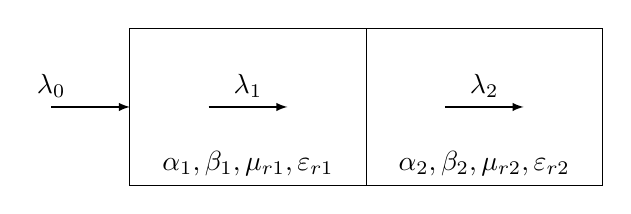
\begin{tikzpicture}
        %arrows
        \draw[-latex](0,1)--(1,1) node at (0,1)[above]{$\lambda_0$};
        \draw[-latex](2,1)--(3,1) node [midway, above]{$\lambda_1$};
        \draw[-latex](5,1)--(6,1) node [midway, above]{$\lambda_2$};

        %frame
        \draw[-](1,0)--(4,0) node [midway, above]{$\alpha_1, \beta_1, \mu_{r1}, \varepsilon_{r1}$};
        \draw[-](4,0)--(7,0) node [midway, above]{$\alpha_2, \beta_2, \mu_{r2}, \varepsilon_{r2}$};
        \draw[-](1,2)--(7,2);
        \draw[-](1,0)--(1,2);
        \draw[-](4,0)--(4,2);
        \draw[-](7,0)--(7,2);
    \end{tikzpicture}
\end{center}
% 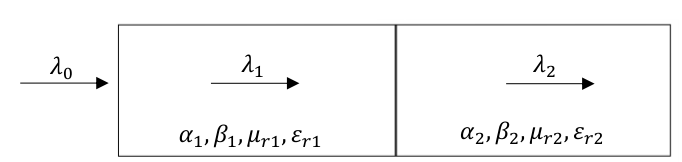
\includegraphics[width=\columnwidth]{Figures/UebergangzweiDielektrika.png}
\begin{align*}
    \quad \qquad \lambda_1 & = \dfrac{\lambda_0}{\sqrt{\mu_{r1}\varepsilon_{r1}}}          & \lambda_2 & = \dfrac{\lambda_0}{\sqrt{\mu_{r2}\varepsilon_{r2}}}                                     \\
    \quad \qquad           &                                                               &           & = \dfrac{\lambda_1\cdot\sqrt{\mu_{r1}\varepsilon_{r1}}}{\sqrt{\mu_{r2}\varepsilon_{r2}}} \\
    \quad \qquad \beta_1   & = \dfrac{2\pi}{\lambda_0}\cdot\sqrt{\mu_{r1}\varepsilon_{r1}} & \beta_2   & = \dfrac{2\pi}{\lambda_0}\cdot\sqrt{\mu_{r2}\varepsilon_{r2}}                            \\
    \quad \qquad Z_{F1}    & = \dfrac{Z_{F0}}{\sqrt{\mu_{r1}\varepsilon_{r1}}}             & Z_{F2}    & = \dfrac{Z_{F0}}{\sqrt{\mu_{r2}\varepsilon_{r2}}}
\end{align*}

\subsection{Energie und Poyntingvektor (Energieflussdichte)}
\begin{align*}
     & \vec{S}                        & = & \vec{E}\times\vec{H} \qquad \si{\left[\frac{W}{m^2}\right]} \\
     & S                              & = & \frac{1}{2} \cdot E \cdot H =                               \\
     &                                & = & \frac{1}{2} \cdot \dfrac{E^2}{Z_{F0}} =                     \\
     &                                & = & \frac{1}{2} \cdot H^2 \cdot Z_{F0}                          \\
     & \overline{S}_{\texttt{Mittel}} & = & \frac{1}{2} \cdot Re\{\vec{E}\times\vec{H}^*\}              \\
     & S                              & = & \dfrac{P}{A_\texttt{Fläche}}                                \\
\end{align*}

\subsubsection{Leistung}

\begin{align*}
    W_{M} & = 1/_2\cdot\mu\cdot H^2         \\
    W_{E} & = 1/_2\cdot\varepsilon\cdot E^2
\end{align*}

\subsubsection{Leistung nach Dämpfung}

\begin{align*}
    P_1 & = P_0 \cdot e^{-2\alpha z}
\end{align*}

\subsubsection{Leistung vom Kabel transportiert}

\begin{align*}
    P & = \dfrac{\hat{U}^2}{2 Z_L}
\end{align*}

\subsection{dÀlembertsche Gleichung (allg.)}
\begin{align*}
    \Delta \vec{E}-\kappa \mu \frac{\partial \vec{E}}{\partial t}-\varepsilon \mu \frac{\partial^{2} \vec{E}}{\partial t^{2}} & = \operatorname{grad} \frac{\rho}{\varepsilon} \\
    \Delta \vec{H}-\kappa \mu \frac{\partial \vec{H}}{\partial t}-\varepsilon \mu \frac{\partial^{2} \vec{H}}{\partial t^{2}} & = 0
\end{align*}

Isolator, ideales Dielektrikum, Nichtleiter $\kappa = 0$
\begin{align*}
    \Delta \vec{E} & =\varepsilon \mu \frac{\partial^{2} \vec{E}}{\partial t^{2}}+\operatorname{grad} \frac{\rho}{\varepsilon} \\
    \Delta \vec{H} & =\varepsilon \mu \frac{\partial^{2} \vec{H}}{\partial t^{2}}
\end{align*}

sehr gute Leiter
\begin{align*}
    \Delta \vec{E} & =\kappa \mu \frac{\partial \vec{E}}{\partial t}+\operatorname{grad} \frac{\rho}{\varepsilon} \\
    \Delta \vec{H} & =\kappa \mu \frac{\partial \vec{H}}{\partial t}
\end{align*}

\subsection{Helmholtz-Gleichungen (Frequenzbereich)}
\begin{align*}
    \Delta \underline{\vec{E}}-\left(\kappa \mu \cdot \mathrm{j} \omega-\varepsilon \mu \cdot \omega^{2}\right) \cdot \underline{\vec{E}} & = \operatorname{grad} \frac{\rho}{\varepsilon} \\
    \Delta \underline{\vec{H}}-\left(\kappa \mu \cdot \mathrm{j} \omega-\varepsilon \mu \cdot \omega^{2}\right) \cdot \underline{\vec{H}} & = 0
\end{align*}

\subsubsection{Zeitbereich}
\begin{align*}
    \Delta \vec{E}-\varepsilon \mu \frac{\partial^{2} \vec{E}}{\partial t^{2}} & =0 \\
    \Delta \vec{H}-\varepsilon \mu \frac{\partial^{2} \vec{H}}{\partial t^{2}} & =0
\end{align*}

\subsubsection{Frequenzbereich (harmonisch)}
\begin{align*}
    \Delta \underline{\vec{E}}+\varepsilon \mu \omega^{2} \cdot \underline{\vec{E}} & =0 \\
    \Delta \underline{\vec{H}}+\varepsilon \mu \omega^{2} \cdot \underline{\vec{H}} & =0
\end{align*}

\textbf{Zeitabhängigkeit harmonisch:}
\begin{align*}
    \Delta \vec{H}   & = (j \omega \mu \sigma - \omega^2 \varepsilon \mu ) \vec{H}                                  \\
    \Delta \vec{E} i & = (j \omega \mu \sigma - \omega^2 \varepsilon \mu ) \vec{E} + grad \frac{ \rho}{\varepsilon}
\end{align*}

\textbf{keine Raumladung $ \rho = 0$}
\begin{align*}
    \Delta \vec{E} & = (j \omega \mu \sigma - \omega^2 \varepsilon \mu ) \vec{E}
\end{align*}

\textbf{Ebene Wellen}
\begin{align*}
    \Delta \vec{E} & = \frac{ \partial \vec{E}}{ \partial z^2} = j \omega \mu ( \sigma + j \omega \varepsilon) \vec{E} \\
    \Delta \vec{H} & = \frac{ \partial \vec{E}}{ \partial z^2} = j \omega \mu ( \sigma + j \omega \varepsilon) \vec{H}
\end{align*}

%%%%%%%%%%%%%%%%%

\subsection{Wellenzahl}
Im Vakuum: $k_{0}=\frac{\omega}{c_{0}}$
\begin{align*}
    k & = \frac{\omega}{v_{p h}} = \frac{2 \pi f}{v_{p h}} = |\vec{k}|                                                              \\
      & = \frac{\omega \cdot n}{c_{0}} = n \cdot k_{0}=\frac{1}{\sqrt{\mu_{r} \cdot \varepsilon_{r}}} \cdot k_{0}=k_{r} \cdot k_{0}
\end{align*}

\subsection{Wellenlänge}
\begin{align*}
    \lambda   & = \dfrac{\lambda_0}{\sqrt{\mu_r \cdot \varepsilon_r}} = \dfrac{2 \pi}{k} = \dfrac{v_{ph}}{f} = [m] \\
              & = \dfrac{\lambda_0}{n} = \dfrac{2 \pi}{n \cdot k_0}                                                \\
    \lambda_0 & = \dfrac{c_0}{f} = \dfrac{2\pi}{k_0}
\end{align*}

\subsection{Phasengeschwindigkeit}
\[
    \dfrac{d z}{d t} = \upsilon_{ph} = c = \dfrac{\omega}{k} = \frac{1}{\sqrt{ \mu_r \mu_0 \varepsilon_r \varepsilon_0}} \qquad \upsilon_{ph,\texttt{Medium} \leq c_0}
\]

\subsubsection{Gruppengeschwindigkeit}
\[
    \upsilon_{g} = \dfrac{d \omega}{d k} = \dfrac{\textnormal{Wegstück der Wellengruppe}}{\textnormal{Laufzeit der Wellengruppe}}
\]

\subsection{Polarisation}
\begin{tabularx}{0.45\textwidth}{>{\hsize=.27\hsize}X|>{\hsize=.5\hsize}X|>{\hsize=.23\hsize}X}
    Lineare      & wenn der Endpunkt des E–Vektors eine Linie beschreibt & $H$ oder $E$ \\
    \hline
    Elliptische  & Endpunkt des E-Vektors eine Ellipse beschreibt        & $E\neq H$    \\
    \hline
    Kreisförmige & der Endpunkt des E-Vektors einen Kreis beschreibt     & $E = H$      \\
\end{tabularx}

\subsection{Verlustlose Polarisation}
\begin{align*}
    Z_F & = \sqrt{\frac{\mu}{\varepsilon}}                                                                                                                                             \\
    r_s & = \frac{\sqrt{\varepsilon_{r1}}\cdot\cos\theta_i - \sqrt{\varepsilon_{r2}}\cdot\cos\theta_t}{\sqrt{\varepsilon_{r2}}\cdot\cos\theta_t + \sqrt{\varepsilon_{r1}}\cos\theta_i} \\
    t_s & = \frac{2\cdot\sqrt{\varepsilon_{r1}}\cdot\cos\theta_i}{\sqrt{\varepsilon_{r2}}\cdot\cos\theta_t + \sqrt{\varepsilon_{r1}}\cdot\cos\theta_i}                                 \\
    r_p & = \frac{\sqrt{\varepsilon_{r1}}\cdot\cos\theta_t - \sqrt{\varepsilon_{r2}}\cdot\cos\theta_i}{\sqrt{\varepsilon_{r2}}\cdot\cos\theta_i + \sqrt{\varepsilon_{r1}}\cos\theta_t} \\
    t_p & = \frac{2\cdot\sqrt{\varepsilon_{r1}}\cdot\cos\theta_i}{\sqrt{\varepsilon_{r2}}\cdot\cos\theta_i + \sqrt{\varepsilon_{r1}}\cdot\cos\theta_t}
\end{align*}

\subsection{Totalrefexion}
\begin{align*}
    \sin\theta_g & = \frac{n_2}{n_1} = \frac{\sqrt{\varepsilon_{r2}\mu_{r2}}}{\varepsilon_{r1}\mu_{r1}}
\end{align*}

\subsection{Grenzwinkel}
\begin{align*}
    \alpha_g & = \sin^{-1} \left( \sqrt{ \dfrac{\mu_{r1} \varepsilon_{r1}}{\mu_{r2} \varepsilon_{r2}}} \right)
\end{align*}
\subsection{Brewster-/Polarisationswinkel, $r=0$}
\begin{itemize}
    \item Snelliusche Brechungsgesetz
          %\item Grenzwinkel $\alpha_g$
          % \item[--] Brewsterwinkel $\alpha_B$ (Welle transmittiert reflexionsfrei)
          %       \begin{itemize}
          %           \item[\textbullet] Parallele Polarisation (Nur wenn $\mu_{r1} = \mu_{r2}$)
          %           \item[\textbullet] Senkrechte Polarisation (Nur wenn $\varepsilon_{r1} = \varepsilon_{r2}$)
          %       \end{itemize}
    \item Paralleler Reflexionskoeffizient:
          \begin{align*}
              \Aboxed{\mu_{r1}=\mu_{r2}}                                                                                                    \\
              \sin\theta_b & = \sqrt{\frac{\varepsilon_2(\mu_2\varepsilon_1 - \mu_1\varepsilon_2)}{\mu_1(\varepsilon_1^2-\varepsilon_2^2)}} \\
              \tan\theta_b & = \sqrt{\frac{\varepsilon_2}{\varepsilon_1}} = \frac{n_2}{n_1}
          \end{align*}

    \item Senkrechter Reflexionskoeffizient:
          \begin{align*}
              \Aboxed{\varepsilon_{r1}=\varepsilon_{r2}}                                                                    \\
              \sin\theta_b & = \sqrt{\frac{\mu_2(\mu_2\varepsilon_1 - \mu_1\varepsilon_2)}{\varepsilon_1(\mu_2^2-\mu_1^2)}} \\
              \tan\theta_b & = \sqrt{\frac{\mu_2}{\mu_1+\mu_2}}
          \end{align*}
\end{itemize}

\begin{align*}
    \dfrac{\sin \vartheta_{2}}{\sin \vartheta_{1}} = \dfrac{k_{h}}{k_{g}} & = \sqrt{\dfrac{\mu_{r 1} \varepsilon_{r 1}}{\mu_{r 2} \varepsilon_{r 2}}} = \dfrac{n_{1}}{n_{2}} = \dfrac{v_{p h, 2}}{v_{p h, 1}} = \dfrac{\lambda_{2}}{\lambda_{1}} \\
    % \alpha_{Bp}                                                           & = \tan^{-1} \left( \sqrt{ \dfrac{\varepsilon_{r1}}{\varepsilon_{r2}}} \right)                                                                                        \\
    % \alpha_{Bs}                                                           & = \tan^{-1} \left( \sqrt{ \dfrac{\mu_{r1}}{\mu_{r2}}} \right)
\end{align*}
\newpage
\subsection{Senkrechter Einfall $ \theta_h = 0$ }

\begin{center}
    \tikzset{cross/.style={cross out, draw=black, minimum size=2*(#1-\pgflinewidth), inner sep=0pt, outer sep=0pt},
        %     %default radius will be 1pt. 
        cross/.default={3.5pt}}
    \begin{tikzpicture}
        %Kreuz
        \draw[dotted] (-3,0) -- (3,0);
        \draw[-] (0,-2.5) -- (0,2.5)                        node[below left] {Material(1)} 
                                                            node[below right] {Material(2)}
                                                            node at (0,-2.5)[above left] {$\varepsilon_1, \mu_1, \sigma_1$}
                                                            node at (0,-2.5)[above right] {$\varepsilon_2, \mu_2, \sigma_2$};
        %Rücklaufende
        \draw[-latex] (-2,1.5) -- (-3,1.5)                  node[above] {$S_r$};
        \draw[-latex] (-2,1.5) -- (-2,2.5)                  node[above] {$E_r$};
        \draw[-] (-2,1.5) circle (0.15)                     node[below right] {$H_r$};
        \draw(-2,1.5) node [cross] {};
        \draw[dotted] (-3,1.5) -- (0,1.5);

        %Hinlaufende
        \draw[dotted] (-3,-1.5) -- (0,-1.5);
        \draw[-latex] (-2,-1.5) -- (-1,-1.5)                node[above left] {$S_h$};
        \draw[-latex] (-2,-1.5) -- (-2,-0.5)                node[above] {$E_h$};
        \draw[-] (-2,-1.5) circle (0.15)                    node[below right] {$H_h$};
        \draw[-,fill=black!100] (-2,-1.5) circle (0.05);

        %Transmitierte
        \draw[-latex] (2,0) -- (3,0)                        node[right] {$S_t$};
        \draw[-latex] (2,0) -- (2,1)                        node[below right] {$E_t$};
        \draw[-] (2,0) circle (0.15)                        node[below right] {$H_t$};
        \draw[-,fill=black!100] (2,0) circle (0.05);
    \end{tikzpicture}
\end{center}

\begin{align*}
    t  = \frac{2 \cdot Z_{F2}}{Z_{F1} + Z_{F2}}\qquad r  = \frac{Z_{F2} - Z_{F1}}{Z_{F1} + Z_{F2}} \\
    \qquad = \frac{\sqrt{\varepsilon_{r2}}-\sqrt{\varepsilon_{r1}}}{\sqrt{\varepsilon_{r2}}+\sqrt{\varepsilon_{r1}}}
\end{align*}

\begin{align*}
    0<t<2 \qquad 0<|r|<1
\end{align*}

Elektrisches Feld:


\begin{align*}
    E_t & = t \cdot E_h \\
    E_r & = r \cdot E_h
\end{align*}

\begin{align*}
    %\vec{E_t}    & = \vec{E_h} + \vec{E_r} \\
    E_t          & = E_h + E_r             \\
    t\cdot E_{h} & = E_{h} + r\cdot  E_{h} \\
    t            & = 1+ r
\end{align*}

Magnetisches Feld:

% \begin{align*}
%     r_m & = r = r_e                                                    \\
%     t_m & = \frac{2}{1+\sqrt{^{\varepsilon_{r1}}/_{\varepsilon_{r2}}}}
% \end{align*}

\begin{align*}
    H_t & = t \cdot H_h \\
    H_r & = r \cdot H_h
\end{align*}

\begin{align*}
    %\vec{H_t}                   & = \vec{H_h}-\vec{H_r}                                \\
    H_t                         & = H_h + H_r                                          \\
    \frac{t\cdot E_{h}}{Z_{F2}} & = \frac{E_{h}}{Z_{F1}} - \frac{r\cdot E_{h}}{Z_{F1}} \\
    \frac{t}{Z_{F2}}            & = \frac{1}{Z_{F1}} - \frac{r}{Z_{F1}}
\end{align*}




\subsubsection{Senkrechter Einfall ideales/verlustl. Dielekt. $\sigma = 0$}

%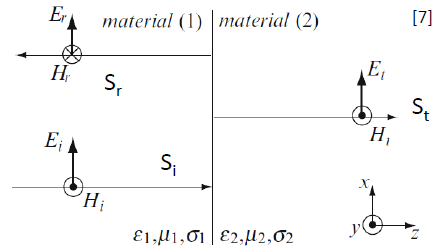
\includegraphics[width=\columnwidth]{Figures/senkrechterEinfall.png}

\begin{align*}
    reel: Z_F        & = \sqrt{\frac{\mu}{\varepsilon}}   \\
    imaginär: \gamma & = j \omega \sqrt{ \mu \varepsilon}
\end{align*}

\begin{align*}
    r & = \frac{Z_{F2} - Z_{F1}}{Z_{F1} + Z_{F2}} = \frac{\sqrt{\frac{\mu_2}{\varepsilon_2}} - \sqrt{\frac{\mu_1}{\varepsilon_1}}}{\sqrt{\frac{\mu_2}{\varepsilon_2}} + \sqrt{\frac{\mu_1}{\varepsilon_1}}} \\
    t & = \frac{2 Z_{F2}}{Z_{F1} + Z_{F2}} = \frac{2\sqrt{\varepsilon_{r1}\mu_{r2}}}{\sqrt{\varepsilon_{r1}\mu_{r2}}+\sqrt{\varepsilon_{r2}\mu_{r1}}}
\end{align*}

% \begin{tabularx}{\columnwidth}{>{\hsize=.35\hsize}X|>{\hsize=.32\hsize}X>{\hsize=.18\hsize}X>{\hsize=.18\hsize}X}
%     idealer Leiter    & $ Z_{F2} = 0 $                    & $ r = -1 $ & $t = 0$ \\
%     \hline
%     ideales Dielektr. & $\mu_{r1} = \varepsilon_{r1} = 1$ &            &         \\
% \end{tabularx}

\subsubsection{Spezialfall $\underline{Medium 1}$ ist Luft}
\begin{align*}
    \Aboxed{ & \mu_{r1} = \varepsilon_{r1} = 1}                                                            \\
    r        & = \frac{\sqrt{\mu_{r2}}-\sqrt{\varepsilon_{r2}}}{{\sqrt{\mu_{r2}}+\sqrt{\varepsilon_{r2}}}} \\
    t        & = \frac{2\sqrt{\mu_{r2}}}{\sqrt{\mu_{r2}}+\sqrt{\varepsilon_{r2}}}
\end{align*}

\subsubsection{Spezialfall $\underline{Medium 2}$ ist Luft}
\begin{align*}
    \Aboxed{ & \mu_{r2} = \varepsilon_{r2} = 1}                                                            \\
    r        & = \frac{\sqrt{\varepsilon_{r1}}-\sqrt{\mu_{r1}}}{{\sqrt{\varepsilon_{r1}}+\sqrt{\mu_{r1}}}} \\
    t        & = \frac{2\sqrt{\varepsilon_{r1}}}{\sqrt{\mu_{r1}}+\sqrt{\varepsilon_{r1}}}
\end{align*}

\subsubsection{Spezialfall $\underline{beide Medien}$ NICHT magnetisch}
\begin{align*}
    \Aboxed{ & \mu_{r1} = \mu_{r2} = 1}                                                                                    \\
    r        & = \frac{\sqrt{\varepsilon_{r1}}-\sqrt{\varepsilon_{r2}}}{{\sqrt{\varepsilon_{r1}}+\sqrt{\varepsilon_{r2}}}} \\
    t        & = \frac{2\sqrt{\varepsilon_{r1}}}{\sqrt{\varepsilon_{r1}}+\sqrt{\varepsilon_{r2}}}
\end{align*}

\subsubsection{Spezialfall $\underline{Medium 2}$ idealer Leiter}
\begin{align*}
    Z_{F2}       & = 0                                 \\
    r            & = -1                                \\
    t            & = 0                                 \\
    \overline{S} & = 0                                 \\
    E_1          & = -2j\cdot E_h\cdot \sin(\beta_1 z) \\
    H_1          & = 2\cdot H_h\cdot \cos(\beta_1 z)
\end{align*}
\begin{align*}
     & \underline{Stehende Welle}                                              \\
     & \rightarrow \text{$H_{max}$ und $E_{min}$ bei } n \cdot \lambda/_2      \\
     & \rightarrow \text{$H_{min}$ und $E_{max}$ bei } (2n-1) \cdot \lambda/_4 \\
     & \qquad \rightarrow 90^\circ Phasenverschiebung
\end{align*}

\subsection{Stehwellenverhältnis}
\[
    \mathrm{SWR} = \frac{E_{\max}}{E_{\min}}=\frac{H_{\max}}{H_{\min}}=\frac{E_{h}+E_{r}}{E_{h}-E_{r}} = \frac{1+|r|}{1-|r|} \quad 1<s<\infty
\]

\newpage
\subsection{Senkrechte Polarisation}
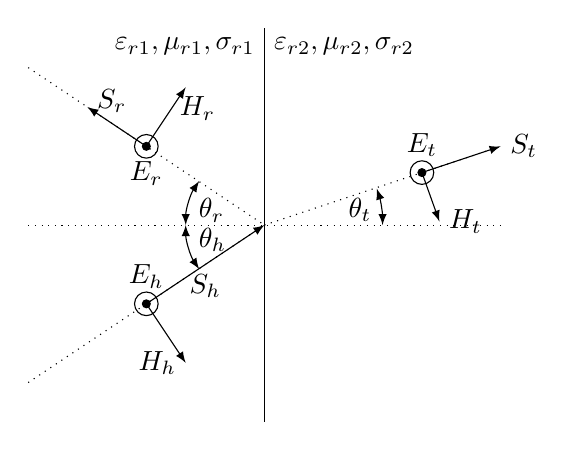
\begin{tikzpicture}
    \tikzset{cross/.style={cross out, draw=black, minimum size=2*(#1-\pgflinewidth), inner sep=0pt, outer sep=0pt},
        %     %default radius will be 1pt. 
        cross/.default={3.5pt}}
    %Kreuz
    \draw[dotted] (-3,0) -- (3,0);
    \draw[-] (0,-2.5) -- (0,2.5)                
        node[below right]   {$\varepsilon_{r2}, \mu_{r2}, \sigma_{r2}$}
        node[below left]    {$\varepsilon_{r1}, \mu_{r1}, \sigma_{r1}$};
    %Rücklaufende
    \draw[-latex] (-1.5,1) -- (-2.25,1.5)   node[right, yshift=.5ex]{$S_r$};
    \draw[-latex] (-1.5,1) -- (-1,1.75)     node[below, xshift=1ex] {$H_r$};
    \draw[-] (-1.5,1) circle (0.15)         node[below,yshift=-.5ex]{$E_r$};
    \draw[-,fill=black!100] (-1.5,1) circle (0.05);
    \draw[dotted] (-3,2) -- (0,0);
    \draw[latex-latex] (146:1) arc (146:180:1) 
        node[midway, right, yshift=-.7ex] {$\theta_r$};

    %Hinlaufende
    \draw[-latex] (-1.5,-1) -- (0,0)        node[below, midway]         {$S_h$};
    \draw[-latex] (-1.5,-1) -- (-1,-1.75)   node[left]                  {$H_h$};
    \draw[-] (-1.5,-1) circle (0.15)        node[above, yshift=.5ex]    {$E_h$};
    \draw[-,fill=black!100] (-1.5,-1) circle (0.05);
    \draw[dotted] (-3,-2) -- (0,0);
    \draw[latex-latex] (180:1) arc (180:214:1)
        node[midway, right, yshift=.7ex] {$\theta_h$};

    %Transmitierte
    \draw[-latex] (2,0.6666) -- (3,1)           node[right] {$S_t$};
    \draw[-latex] (2,0.6666) -- (2.2223,0.0448) node[right] {$H_t$};
    \draw[-] (2,0.6666) circle (0.15)           node[above, yshift=.5ex] {$E_t$};
    \draw[-,fill=black!100] (2,0.6666) circle (0.05);
    \draw[dotted] (0,0) -- (3,1);
    \draw[latex-latex] (0:1.5) arc (0:18:1.5)
        node[midway, left, yshift=-.3ex] {$\theta_t$};

\end{tikzpicture}

\[ \boxed{\texttt{mit } Z_{F0} = 120\pi \approx 377\si{\ohm}} \]
\begin{align*}
    Z_{Fn}                & = Z_{F0}\cdot\frac{1}{\sqrt{\varepsilon_{rn}}}            \\
    \frac{Z_{F1}}{Z_{F2}} & = \frac{\sqrt{\varepsilon_{r2}}}{\sqrt{\varepsilon_{r1}}}
\end{align*}
\[ n: \texttt{Brechungsindex} \quad ; \quad \theta_h = \theta_r\]
\begin{align*}
    \frac{\sin\theta_t}{\sin\theta_h} & = \frac{\lambda_2}{\lambda_1}= \frac{\beta_1}{\beta_2}= \frac{n_1}{n_2} \\
    \sin\theta_t                      & = \sqrt{\frac{\varepsilon_{r1}}{\varepsilon_{r2}}}\cdot \sin\theta_h
\end{align*}

\begin{itemize}
    \item magnetischer/elektrischer Reflexionsfaktor $[1]$
    \item magnetischer Transmissionsfaktor $[1]$
    \item elektrischer Transmissionsfaktor $[1]$
\end{itemize}
\begin{align*}
    r_s     & =  r_{e s} = r_{m s} =                                                                                                                                          \\
            & = \frac{Z_{F 2} \cdot \cos \theta_h-Z_{F 1} \cdot \cos \theta_t}{Z_{F 2} \cdot \cos \theta_h+Z_{F 1} \cdot \cos \theta_t}                                       \\
            & = \frac{\cos\theta_h-\sqrt{^{\varepsilon_{r2}}/_{\varepsilon_{r1}}-\sin^2\theta_h}}{\cos\theta_h+\sqrt{^{\varepsilon_{r2}}/_{\varepsilon_{r1}}-\sin^2\theta_h}} \\
    t_{m s} & = Z_{F 1} \cdot \frac{2 \cdot \cos \theta_h}{Z_{F 2} \cdot \cos \theta_h+Z_{F 1} \cdot \cos \theta_t}                                                           \\
            & = (1 - r_{s}) \cdot \dfrac{\cos \theta_h}{\cos \theta_t}                                                                                                        \\
            & = \frac{Z_{F1}}{Z_{F2}}\cdot t_{es}                                                                                                                             \\
    t_{e s} & = Z_{F 2} \cdot \frac{2 \cdot \cos \theta_h}{Z_{F 2} \cdot \cos \theta_h+Z_{F 1} \cdot \cos \theta_t}                                                           \\
            & = 1+r_{s}
\end{align*}

\begin{align*}
    E_{r} & = r_{s} \cdot E_{h}   \\
    E_{t} & = t_{e s} \cdot E_{h} \\
    H_{r} & = r_{s} \cdot H_{h}   \\
    H_{t} & = t_{m s} \cdot H_{h}
\end{align*}

\subsection{Parallel Polarisation}
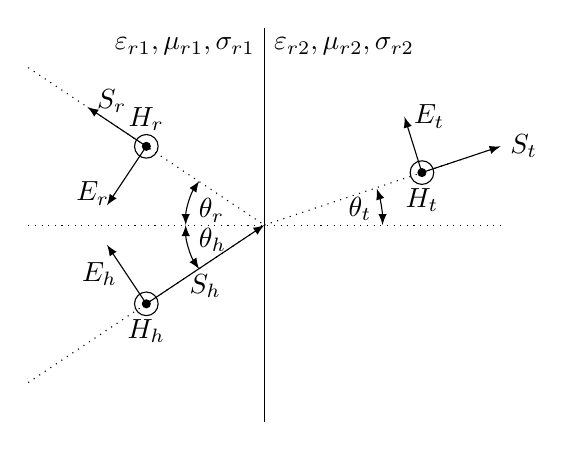
\begin{tikzpicture}
    \tikzset{cross/.style={cross out, draw=black, minimum size=2*(#1-\pgflinewidth), inner sep=0pt, outer sep=0pt},
        %     %default radius will be 1pt. 
        cross/.default={3.5pt}}
    %Kreunz
    \draw[dotted] (-3,0) -- (3,0);
    \draw[-] (0,-2.5) -- (0,2.5) node[below right] {$\varepsilon_{r2}, \mu_{r2}, \sigma_{r2}$}
        node[below left] {$\varepsilon_{r1}, \mu_{r1}, \sigma_{r1}$};
 
    %Hinlaufende
    \draw[-latex] (-1.5,-1) -- (0,0) node[below, midway ]       {$S_h$};
    \draw[-latex] (-1.5,-1) -- (-2,-0.25) node[left, midway]    {$E_h$};
    \draw[-] (-1.5,-1) circle (0.15) node[below,yshift=-.5ex]   {$H_h$};
    \draw[-,fill=black!100] (-1.5,-1) circle (0.05);
    \draw[dotted] (-3,-2) -- (0,0);
    \draw[latex-latex] (180:1) arc (180:214:1)
        node[midway, right, yshift=.7ex] {$\theta_h$};

    %Rücklaufende
    \draw[-latex] (-1.5,1) -- (-2.25,1.5) node[right, yshift=.5ex]          {$S_r$};
    \draw[-latex] (-1.5,1) -- (-2,0.25) node[left, yshift=1ex, xshift=1ex]  {$E_r$};
    \draw[-] (-1.5,1) circle (0.15) node[above, yshift=.5ex]                {$H_r$};
    \draw[-,fill=black!100] (-1.5,1) circle (0.05);
    \draw[dotted] (-3,2) -- (0,0);
    \draw[latex-latex] (146:1) arc (146:180:1)
        node[midway, right, yshift=-.7ex] {$\theta_r$};

    %Transmitierte
    \draw[-latex] (2,0.6666) -- (3,1) node[right]                   {$S_t$};
    \draw[-latex] (2,0.6666) -- (1.7777,1.378)  node[right]         {$E_t$};
    \draw[-] (2,0.6666) circle (0.15) node[below, yshift=-0.5ex]    {$H_t$};
    \draw[-,fill=black!100] (2,0.6666) circle (0.05);
    \draw[dotted] (0,0) -- (3,1);
    \draw[latex-latex] (0:1.5) arc (0:18:1.5)
        node[midway, left, yshift=-.7] {$\theta_t$};

\end{tikzpicture}

\[ \boxed{\texttt{mit } Z_{F0} = 120\pi \approx 377\si{\ohm}} \]
\begin{align*}
    Z_{Fn}                & = Z_{F0}\cdot\frac{1}{\sqrt{\varepsilon_{rn}}}            \\
    \frac{Z_{F1}}{Z_{F2}} & = \frac{\sqrt{\varepsilon_{r2}}}{\sqrt{\varepsilon_{r1}}}
\end{align*}
\[ n: \texttt{Brechungsindex} \quad ; \quad \theta_h = \theta_r\]
\begin{align*}
    \frac{\sin\theta_t}{\sin\theta_h} & = \frac{\lambda_2}{\lambda_1}= \frac{\beta_1}{\beta_2}= \frac{n_1}{n_2} \\
    \sin\theta_t                      & = \sqrt{\frac{\varepsilon_{r1}}{\varepsilon_{r2}}}\cdot\sin\theta_h
\end{align*}

\begin{itemize}
    \item magnetischer/elektrischer Reflexionsfaktor $[1]$
    \item magnetischer Transmissionsfaktor $[1]$
    \item elektrischer Transmissionsfaktor $[1]$
\end{itemize}
\begin{align*}
    r_p     & =  r_{e p} = r_{m p} =                                                                                                                                                                                                      \\
            & = \frac{Z_{F 2} \cdot \cos \theta_t-Z_{F 1} \cdot \cos \theta_h}{Z_{F 2} \cdot \cos \theta_t+Z_{F 1} \cdot \cos \theta_h} =                                                                                                 \\
            & = \frac{\varepsilon_{r2}\cos\theta_h-\sqrt{\varepsilon_{r2}\varepsilon_{r1}-{\varepsilon_{r1}}^2\sin^2\theta_h}}{\varepsilon_{r2}\cos\theta_h+\sqrt{{\varepsilon_{r2}\varepsilon_{r1}-{\varepsilon_{r1}}^2\sin^2\theta_h}}} \\
    t_{e p} & = Z_{F 2} \cdot \frac{2 \cdot \cos \theta_h}{Z_{F 1} \cdot \cos \theta_h+Z_{F 2} \cdot \cos \theta_t}                                                                                                                       \\
            & = (1 + r_{p}) \cdot \dfrac{\cos \theta_h}{\cos \theta_t}                                                                                                                                                                    \\
            & = \frac{Z_{F2}}{Z_{F1}}\cdot t_{mp}                                                                                                                                                                                         \\
    t_{m p} & = Z_{F 1} \cdot \frac{2 \cdot \cos \theta_h}{Z_{F 1} \cdot \cos \theta_h+Z_{F 2} \cdot \cos \theta_t}                                                                                                                       \\
            & = 1+r_{p}
\end{align*}

\begin{align*}
    E_{r} & = r_{s} \cdot E_{h}   \\
    E_{t} & = t_{e s} \cdot E_{h} \\
    H_{r} & = r_{s} \cdot H_{h}   \\
    H_{t} & = t_{m s} \cdot H_{h} \\
\end{align*}


